\section{Pedidos fuera de la cocina}
Como dijimos este componente tiene por responsabilidad el manejo de la vida de los pedidos que estan fuera de la cocina (por cocina entendemos no solo al horno, sino tambi�n a la preparaci�n de los pedidos).

Nuestra idea fue tener un coordinadorDePedidos que siga el patron Fa�ade, de modo que muestre a la interfaz grafica una intrefaz \textit{``gruesa''} con las funciones que se realizan dentro del componente. Esta clase no va a tener gran inteligencia, sino que se limitara a propagar la llamada originada por la interfaz grafica a la clase responsable de manejar esa llamada. As�, por ejemplo para ver el estado de un pedido o ingrear un nuevo pedido se deber� pasar por esta clase.
La idea de esta clase es desacoplar la interfaz grafica de las clases que manejan a los pedidos fuera de la cocina. Si bien esta clase para tener baja cohesi�n, al mirarla de cerca vemos que lo �nico que hace es derivar las llamadas. De este modo si bien a trazo grueso parece tener una interfaz con poca cohesi�n, esta nos permite lograr un menor grado de acoplamiento entre la interfaz y el sistema en si. Por esta raz�n decidimos pese al aparente conflicto con la cohesi�n, decidimos mantener esta clase.
Ademas el coordinadorDePedidos se comunica con el componente encargado de crearPedidos, haciendo de puente entre ambos componentes.
Cuando se realiza un pedido de ingreso, el coordinador se encarga de pedir que se genere el pedido, y en caso de que se pueda crear, lo deriva al controladorDePreIngreso, cuya funci�n es determinar si el pedido debe ir a la cola de listos, porque no hay nada que preparar, ni cocinar, o lo tiene que mandar al controlador de ingreso, porque hay algo que cocinar o preparar. Este comportamiento se hizo con la intenci�n de permitir en un futuro incorporar otros productos ademas de pizzas o empanadas. Por ejemplo, podrian venderse ensaladas, las cuales no requieren de cocci�n, pero si de preparaci�n. Por eso decidimos que un producto tuviera atributos de cocinable y preparable.

El controladorDeIngreso se encarga de mantener la cola de ingreso, asi como de suministrar los pedidos al CoordinadorDeCocina, para que este los distribuya al preparador o al coordinador de horno.
El coordinadorDeIngreso puede recibir recibir una solicitud de un pedido de cierto tipo por parte del CoordinadorDeCocina, por ejemplo puede recibir una solicitud del proximo pedido que contenga algun producto del tipo empanada. 
Por otro lado, cada vez que ingresa un nuevo pedido, el controladorDeIngreso pregunta al CoordinadorDeCocina si puede recibir dicho pedido. Esta funcionalidad sirve para aquellos casos en los que por ejemplo no hay ningun pedido ingresado con empanadas y el maestro empanadero esta ocioso. Si llega un nuevo pedido con empanadas, el maestro debe ser notificado, por esta razon el ControladorDeIngreso pregunta si debe encolar el pedido o hay alguien que lo vaya a preparar.
%FIXME: la parte de preguntar es propia del standard, es decir del concreto

Otra clase de este componente, es el ControladorDeListos, este controlador va a recibir los pedido listos y va a encargarse en el momento del despacho de decidir que hacer con el pedido. Por ejemplo si es un pedido con delivery hay que marcar que salio con el delivery, y si era local hay que marcarlo como finalizado.

La clase controladorDeEntragas contiene a todos los pedidos cuya entrega esta pendiente, y se encargan de finalizar el pedido cuando se notifica la entrega.

Por ultimo el controladorPedidosMesa monitorea los pedidos entregados a una cierta mesa, permitiendo que al cerrar la mesa se fijen sus formas de pago.

La clase controladorDeIngreso es abstracta porque consideramos que la estrategia con la que se maneja la cola de ingreso podria cambiar, de esta manera la versi�n propuesta por nosotros en la etapa de especificaci�n es implementada por controladorDeIngresoStandard. Utilzar una clase abstracta nos permite lograr flexibilidad si se quiere cambiar de politica de manejo de esta cola, por ejemplo usando un manejo del tipo mas corto primero.


\textcolor{Red}{TODO: interacciones de estas clases con la GUI}

\textcolor{Red}{TODO: explicacion de metodos importantes}

% FIXME: esto vuela, lo puse en la intro
\subsection{Modelado de escenarios}


%FIXME: en el ingreso se da a la gui la responsabilidad de mostrar los datos del pedido, tiempo estimado y precio, no se si eso esta bien
\subsubsection{Ingreso de un pedido de solo bebidas}
A continuaci�n intentaremos mostrar las interacciones existentes en este componente con el fin de modelar su comportamiento.
Como primer escenario veamos que ocurre cuando ingresa un pedido de solo bebidas Telefonico. En este caso el pedido ser� creado por el generador de pedidos, sin embargo las interacciones propias de la creaci�n no se detallaran en este escenario, asi como tampoco la validaci�n previa del cliente. Una vez que el pedido es creado, pasa al controlador de pre ingreso que lo examina para decidir si debe ir a la cocina o considerarse un pedido listo. En este caso, como solo hay bebidas, el pedido queda listo. El controlador de listos agrega el pedido a su lista de pedidos, se hace responsable del mismo y cambia su estado. 
Al agregar el pedido a la lista notifica a su observador de que ocurrio un cambio, por ejemplo para que se repinte la lista de pedidos listos.

\begin{figure}[H]
\centering
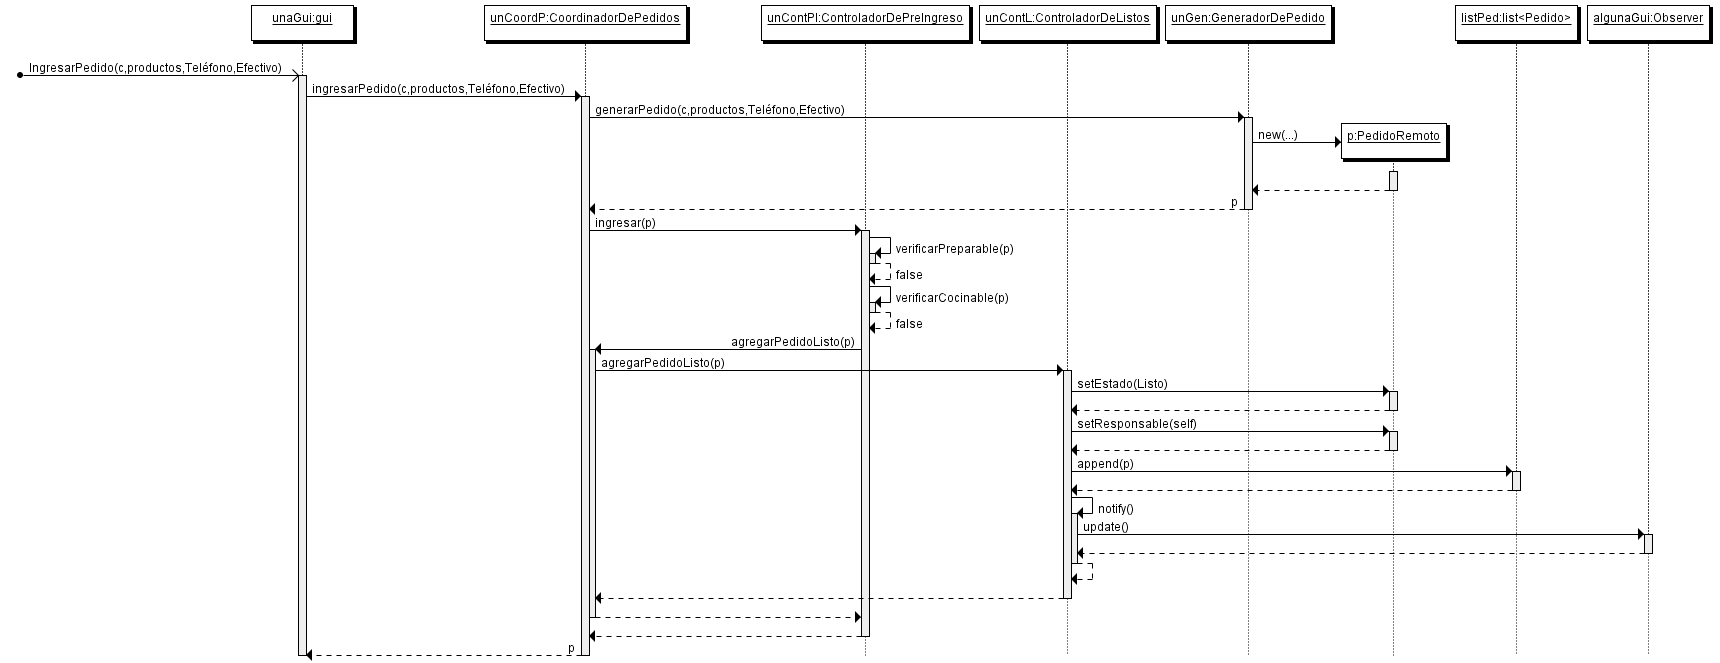
\includegraphics[height=21cm]{./figuras/remotoBebidas.png}
\caption{Ingreso de un pedido remoto de solo bebidas}
\end{figure}

El verifcarPreprable y su analogo para cocinable, basicamente recorren los productos del pedido, buscando si alguno tiene un tipo preparable o cocinable.

\begin{figure}[H]
\centering
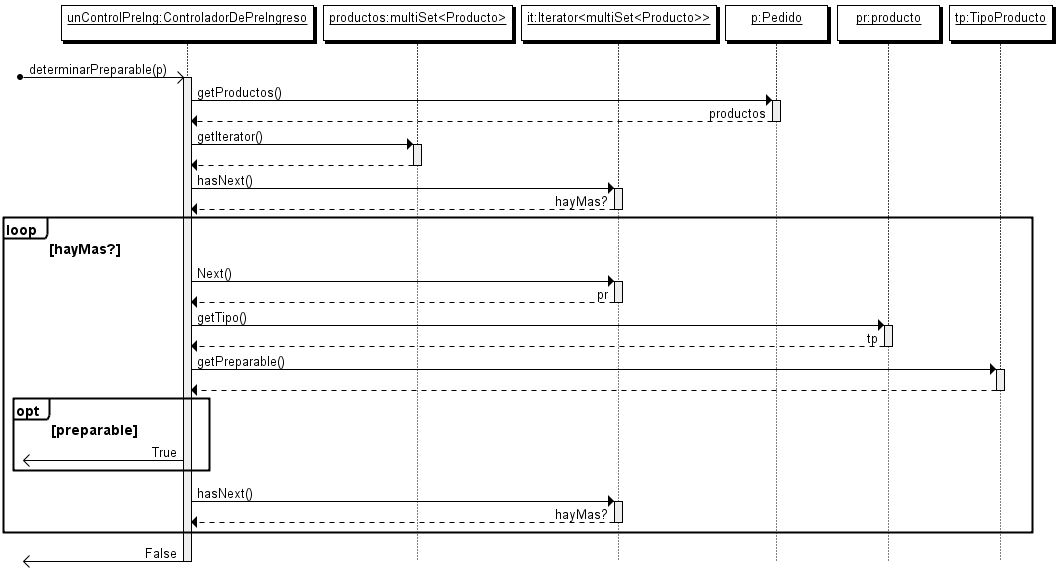
\includegraphics[height=9cm]{./figuras/determinarPreparable.png}
\caption{VerificarPreparable}
\end{figure}

\begin{figure}[H]
\centering
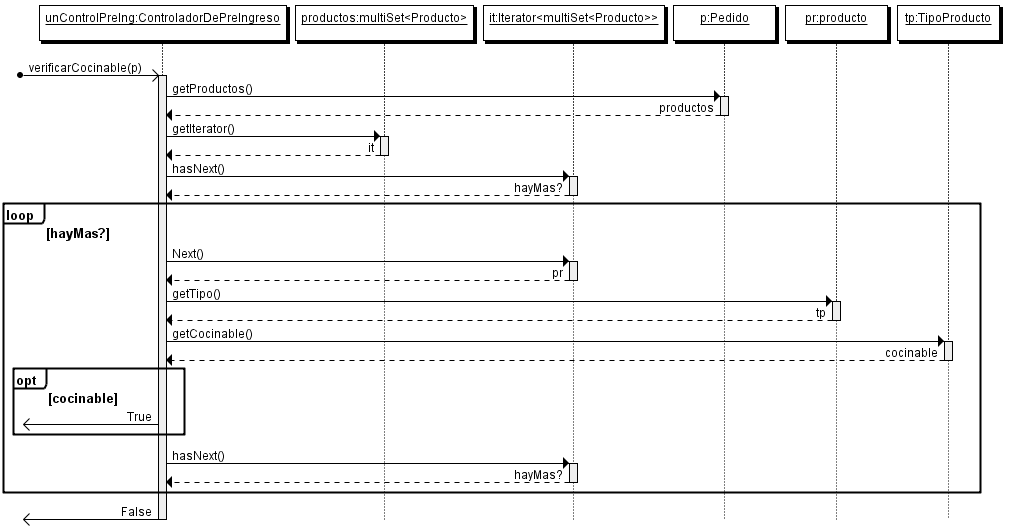
\includegraphics[height=9cm]{./figuras/determinarCocinable.png}
\caption{VerificarCocinable}
\end{figure}
%FIXME: o tocamos la imagen con el inkscape o justifamos las cosas que son de notacion rara

\subsubsection{Ingreso de un pedido con comidas}
De forma analoga al escenario anterior, supongamos que se va a ingresar un pedido, pero en este caso, el pedido si ten�a comidas, por lo que el controlador de pre ingresos se lo va a mandar al de ingresos. Este intenta pasarlo a la cocina para ver si esta puede hacerse cargo del pedido. Esto es asi porque en la especificaci�n se pide que si entra un pedido y el maestro estaba ocioso, se le notifique que prepare el pedido ingresado. Como conocer si los maestros estan preparando algo, no es asunto de este controlador lo que decidimos es que lo pase hacia la cocina y espere respuesta de esta. Modelaremos los dos escenarios, primero el caso en el que la cocina le dice que no puede hacerse cargo y en segundo lugar el caso en el que la cocina si acepta el pedido.

En el primer caso, el controlador de ingresos se hace cargo del pedido, cambiando su estado, marcando el pedido como ingresado y agregandolo a la cola.

\begin{figure}[H]
\centering
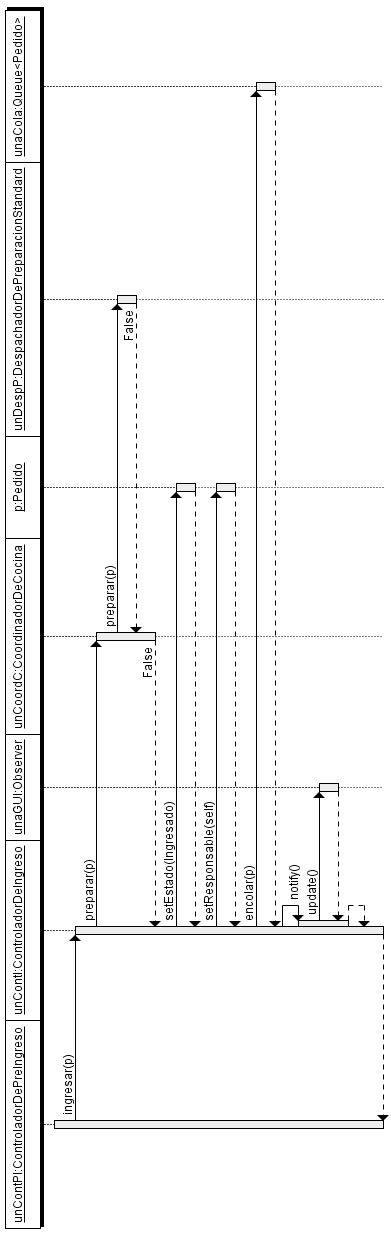
\includegraphics[height=6cm]{./figuras/remotoComidas.png}
\caption{Ingreso de un pedido remoto con comida que queda encolado para su ingreso}
\end{figure}

En el segundo caso, como se va a hacer cargo la cocina, el controlador de ingreso no debe hacer nada cuando se regresa la llamada.

\begin{figure}[H]
\centering
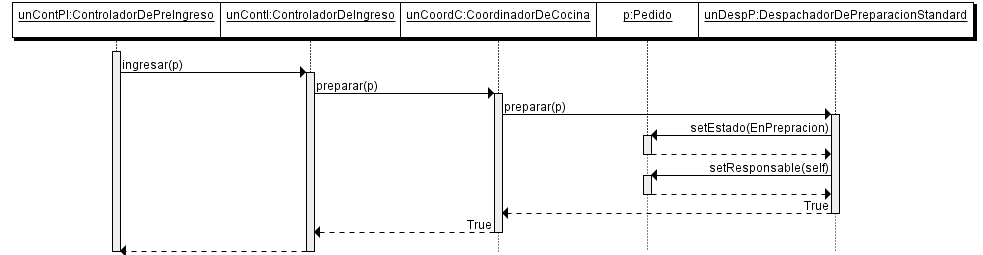
\includegraphics[height=4cm]{./figuras/remotoComidasquedapreparando.png}
\caption{Ingreso de un pedido remoto con comida que pasa a estar preparando}
\end{figure}

\subsubsection{Despacho de un pedido}
Cuando el pedido esta cocinado es responsabilidad de el controlador de listos. Una vez que el pedido esta listo, se puede despachar. Despachar tiene una semantica diferente segun el origen del pedido, por eso es que el controlador posse un despachar para los subtipos remotos, otro para el pedido de mesa y finalmente un tercer despachar para pedidos de mostrador.

En el escenario en el cual el pedido a despachar es de origen remoto, el controlador de listos, lo que hace es sacarlo de la lista, marcarlo como que salio en entrega y avisar de esto al coordinadorDePedido para que avise al controlador de entrega. Ademas notifica a su observador del evento. Esto se hace con la intenci�n de que la gui se entere de que un pedido salio de esta lista y la refresque.

El controlador de entregas pone al pedido en su lista de pedidos, y se asigna como responsable de la cancelaci�n del mismo.

Veamos el diagrama de secuencia comenzando la misma con la llegada de un mensaje de despachar al coordinador de pedidos

\begin{figure}[H]
\centering
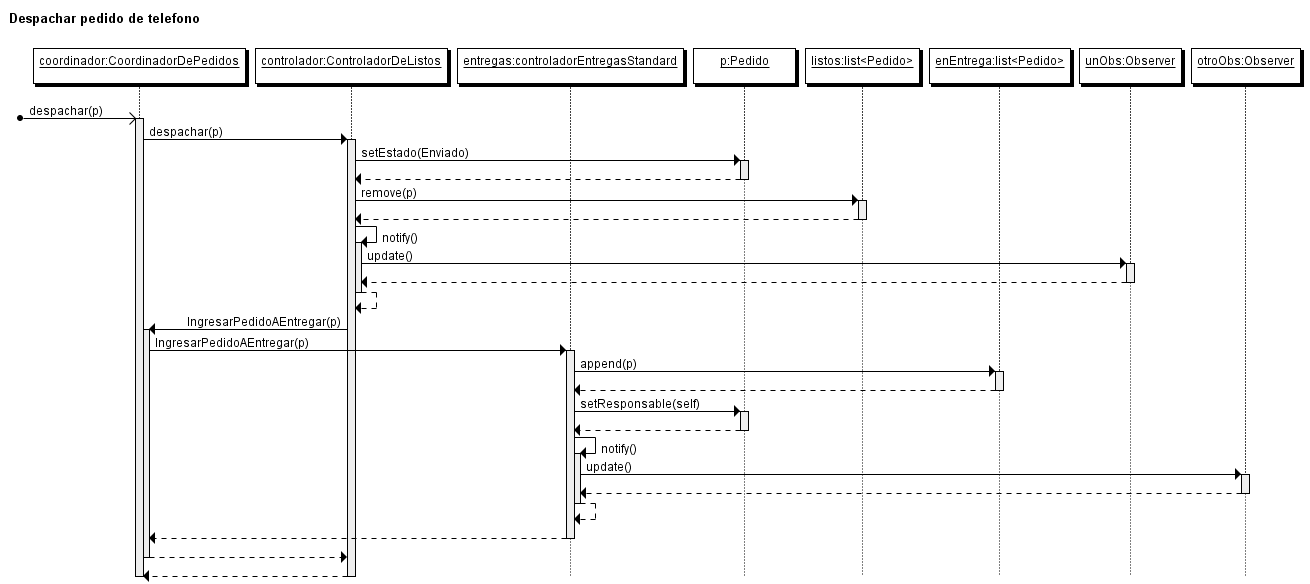
\includegraphics[height=7cm]{./figuras/despacharPedidoTelefono.png}
\caption{Despacho de un pedido telefonico}
\end{figure}

Otro escenario diferente lo constituye el despacho de un pedido de mesa. En este caso, el pedido deja la orbita del controlador de lista, para pasar al controlador de pedidos de mesa, el cual se encargara cuando se cierre la misma de asignar la forma de pago a los pedidos. Este encargado tambi�n se hace cargo de la cancelaci�n. Ambos controladores ademas notifican a su observador de los cambios en su lista.

El diagrama de secuencia es el siguiente:

\begin{figure}[H]
\centering
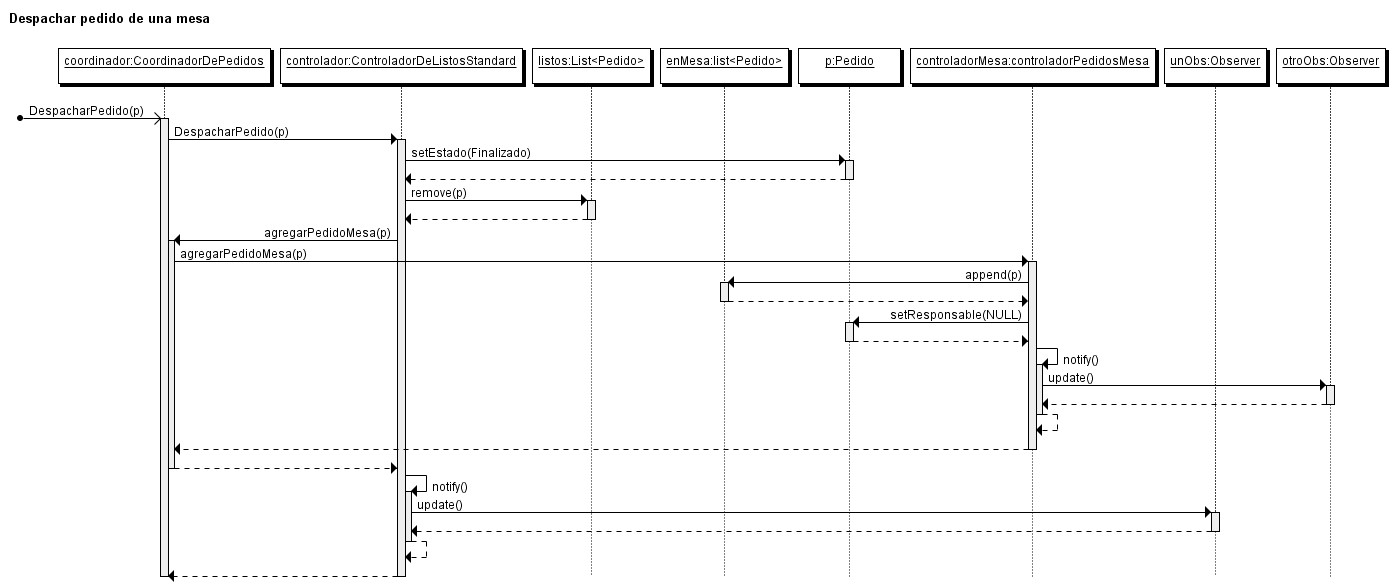
\includegraphics[height=7cm]{./figuras/despacharPedidoMesa.png}
\caption{Despacho de un pedido de mesa}
\end{figure}

Finalmente en el caso de un pedido de mostrador, el controlador de listos solo lo marca como terminado, ya que el pedido fue entregado y se conoce su forma de pago. Por lo tanto la secuencia es la siguiente:

\begin{figure}[H]
\centering
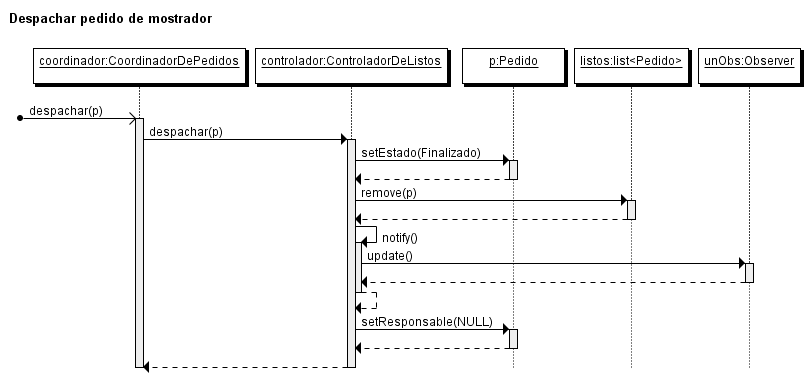
\includegraphics[height=8cm]{./figuras/despacharPedidoMostrador.png}
\caption{Despacho de un pedido de mostrador}
\end{figure}

\subsubsection{Pedido de proximo pedido a preparar}
Cuando el maestro termina de preparar un pedido (o sub pedido) se notifica al sistema. Entonces el despachador se encargado de pedirle al coordinador de la cocina que le consiga un pedido. Este habla con el controlador de ingreso para pedirle el pedido. Modelaremos el escenario en el cual el coordinador pide un pedido al controlador de ingreso. 

Para solicitar un pedido, se suministra al controlador de ingreso un TipoProducto, que le permite realizar la busqueda del primer pedido en la cola que contenga dicho tipo de producto. Esto es util si en un futuro se extienden los tipos de productos, o por ejemplo un maestro pasa a ser capaz de preparar otras cosas.

El controlador de ingreso entonces se encarga de buscar si en su cola hay alguien que cumpla tener algun producto del tipo solicitado. Si lo encuentra lo devuelve, sino devuelve NULL para informar que no tiene ningun pedido que contenga ese producto, por lo que el controlador quedara ocioso.

En el caso de tener que sacar un pedido de la cola, el controlador de listos hace un notify para invocar el update de su observador, por ejemplo para que se redibuje la cola de ingreso.

\begin{figure}[H]
\centering
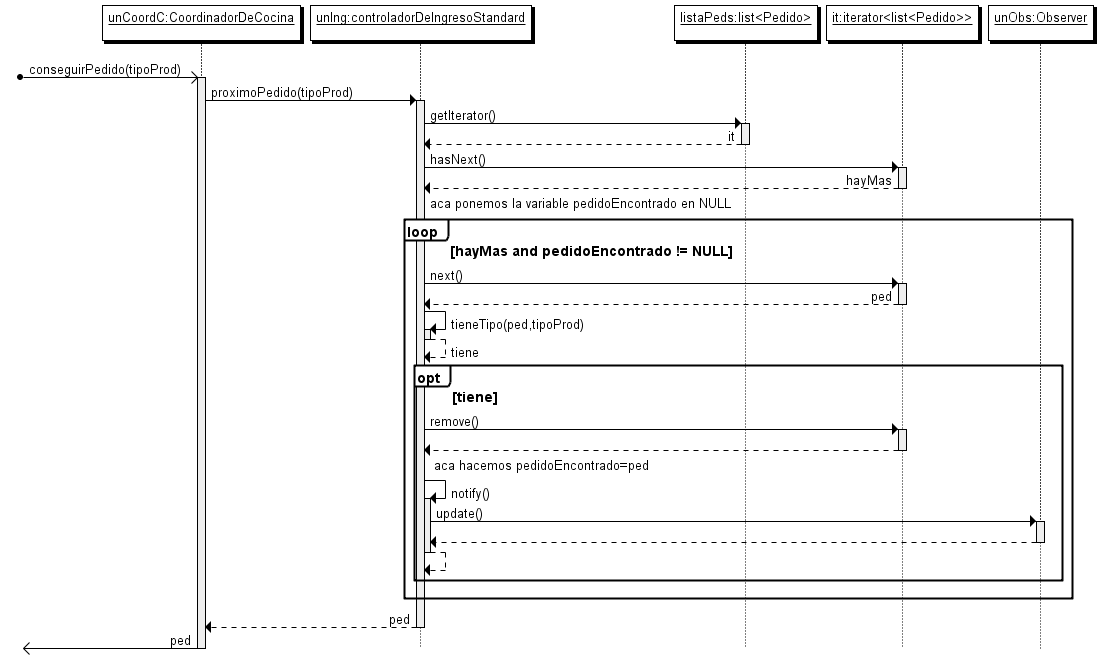
\includegraphics[height=8cm]{./figuras/proximoPedido.png}
\caption{Seleccion del proximo pedido}
\end{figure}

tieneTipo se encarga de recorrer los productos del pedido para ver si hay alguno con un cierto tipo de producto, el siguiente diagrama permite modelar la secuencia desatada por la ejecuci�n de este metodo.

\begin{figure}[H]
\centering
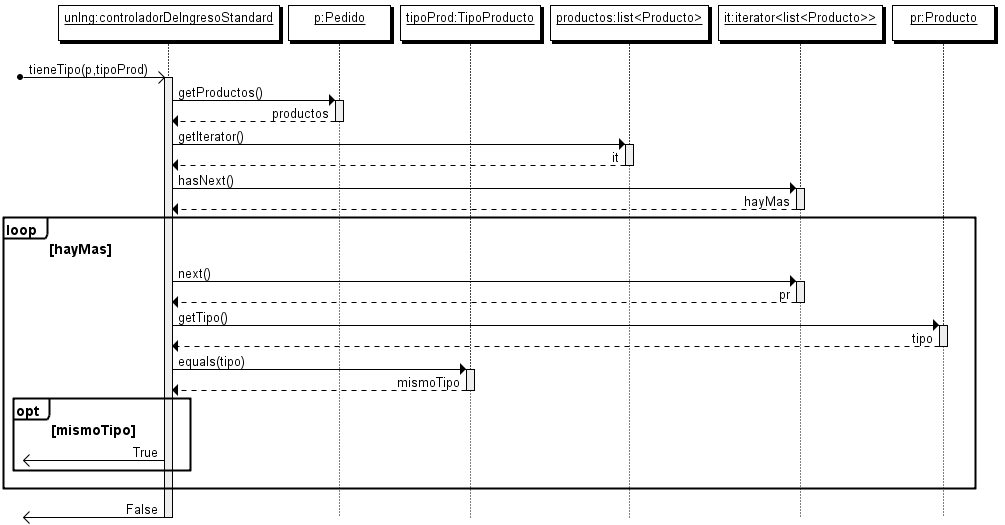
\includegraphics[height=8cm]{./figuras/tieneTipo.png}
\caption{tieneTipo}
\end{figure}

%TODO: decidir aridad de esta funci�n
%TODO: mostrar pseudocodigo

\subsubsection{Notificaci�n de entrega}
Cuando el usuario notifica una entrega, selecciona el pedido de la lista de pedidos con entrega pendiente e indica que fue entregado. Al hacerlo, se notifica al coordinador de pedidos, que pasa la llamada al controlador de entregas. El mismo busca el pedido que debe marcar como finalizado, lo marca y setea en \verb0NULL0 el encargado de cancelaci�n, ya que el pedido no puede ser cancelado a partir de este momento. Luego notifica a su observador que un pedido salio de su cola, por ejemplo para que la GUI que muestra los pedidos con entrega pendiente se refresque.

El escenario donde se notifica la entrega de un pedido, puede modelarse con el siguiente diagrama de secuencia:

\begin{figure}[H]
\centering
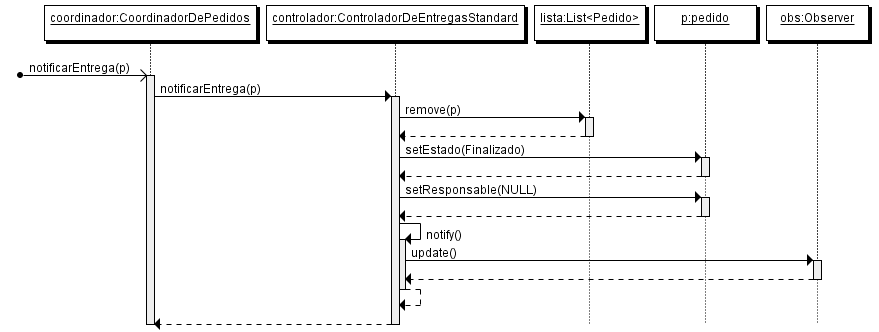
\includegraphics[height=7cm]{./figuras/notificarEntrega.png}
\caption{Notificacion de pedido entregado}
\end{figure}


\subsubsection{Cerrado de mesa}
Para cerrar una mesa el usuario ingresa el numero de mesa que desea cerrar, elegiendo tambi�n la forma de pago. La GUI pasa el mensaje al coordinador de pedidos, el cual propaga la llamada hacia el controlador de mesa, que se va a encargar de completar la forma de pago de los pedidos de la mesa seg�n el parametro pasado y los quita de la lista de pedidos con entrega pendiente. Entonces notifica a su observador de que se modific� su lista de pedidos.

El siguiente diagrama nos permite modelar dicho escenario:

\begin{figure}[H]
\centering
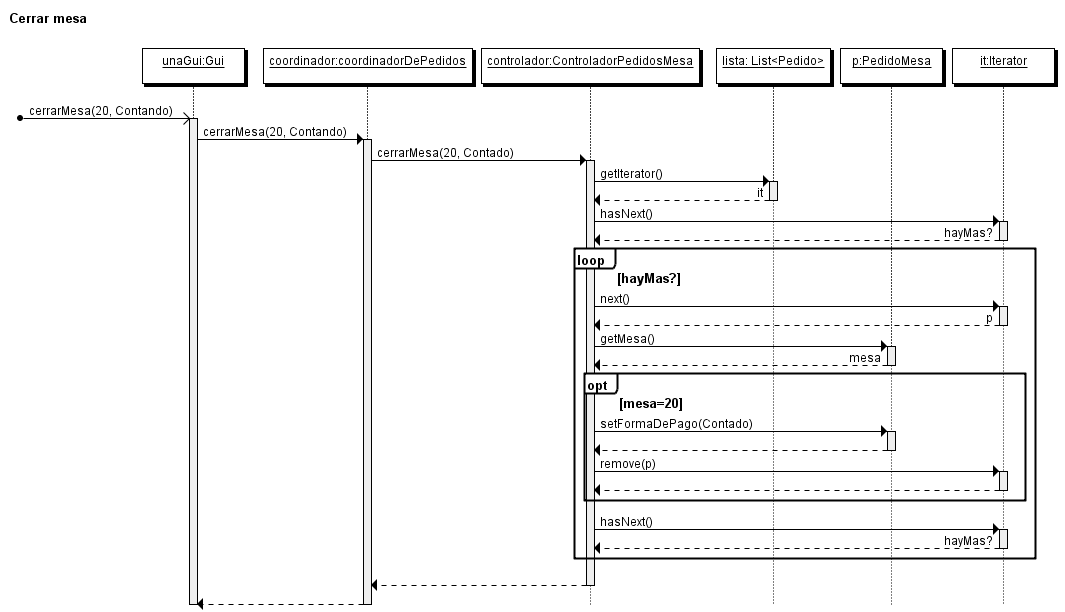
\includegraphics[height=9cm]{./figuras/cerrarMesa.png}
\caption{Cerrado de mesa}
\end{figure}

\subsubsection{Consulta de estado}
Dado que la GUI sabe mostrar pedidos, este escenario queda bastante simple, ya que la interfaz lista los pedidos, permitiendo al encargado filtrar o buscar por ejemplo por cliente o ID. Una vez que el encargado selecciona un pedido, solicita ver el estado y se llama al getEstado del pedido.

\begin{figure}[H]
\centering
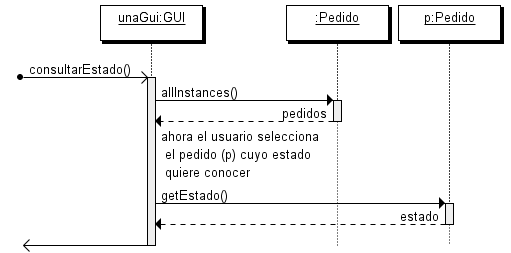
\includegraphics[height=9cm]{./figuras/consultarEstado}
\caption{Notificacion de pedido entregado}
\end{figure}

\subsubsection{Mover un pedido en la cola de ingreso}
Para mover un pedido en la cola de ingreso, la GUI se encarga de pedir la lista de pedidos en ingreso, la muestra y luego el encargado selecciona un pedido y puede elegir entre subir o bajar.

A continuaci�on mostramos un escenario en la que se pide subir un pedido en la cola. Vamos a suponer que el pedido a subir no es el primero, de esta manera nos evitamos usar un alt.

El controlador de pedidos pasa las llamadas al controlador de ingreso, que se encarga de obtener el indice del pedido, sacarlo y volverlo a poner en la posicion inmediatamente superio a la que tenia antes.

\begin{figure}[H]
\centering
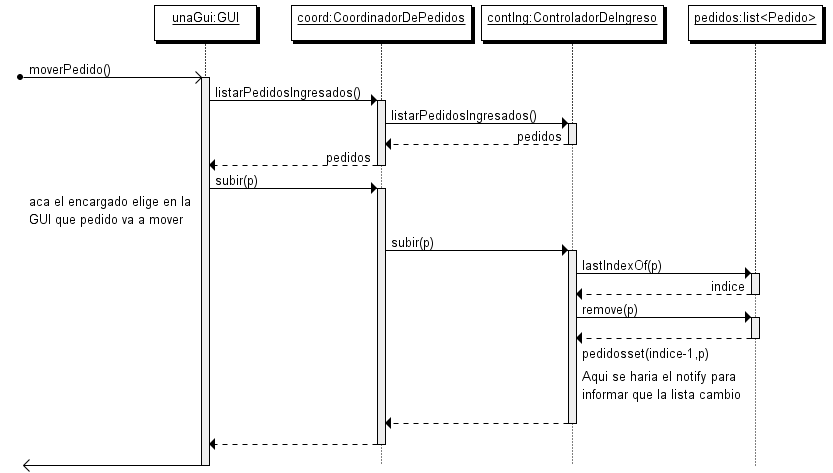
\includegraphics[height=10cm]{./figuras/subirPedido.png}
\caption{Subir un pedido en la cola de ingreso}
\end{figure}
